\ifgerman{\chapter{Grundlagen}}{\chapter{Background}}
\label{background}


In this chapter, we introduce the general terms and definitions that help the reader to understand the remainder of the work. In \hyperref[sec:2.1]{Section 2.1}, we provide a detailed description and definition of the configurable software system along with their use cases. In \hyperref[sec:2.2]{Section 2.2}, we describe the performance and how it is used in this thesis, followed by an example of a performance-influence model and how performance-influence models are derived. In \hyperref[sec:2.3]{Section 2.3}, we describe different visualizations techniques for performance-influence models.


\section{Configurable Software System}
\label{sec:2.1}
A software or a system with different configuration options is called a configurable software system~\cite{DBLP:books/daglib/0032924}. A configuration option offers a specific functionality to the system. For instance, a configuration option \texttt{compression} introduces a functionality to compress files. A configuration option could belong to an \texttt{alternative} group or an \texttt{or} group. The alternative group implies that a configuration option should be selected with exactly one of several algorithms available for that functionality. Whereas, or group implies that the configuration option should be selected with at least one of several algorithms available for that functionality. For instance, the configuration option compression has several algorithms like \texttt{AES, 3DES, SHA1}. Furthermore, configuration options can be optional or mandatory. Optional configuration options can be either selected or deselected, whereas mandatory options are always be selected. Configuration options that can be selected or deselected are called binary configuration options. 

Optional configuration option also means that several of these configuration options can be selected at the same time, but oftenly not all combinations of the configuration options selected together are valid. The validity of the combinations depends on constraints. A constraint is a limitation on how the configuration options can be selected in combination with other configuration options. For instance, two configuration options can be mutually exclusive. When at least one of these constraints is not fulfilled, in a combination, the combination is invalid. The valid combinations of the configuration options is called a \enquote*{configuration}. The configuration options and the constraints among them are described in a variability model. 

Formally, we denote $\mathcal{O}$ as the set of all configuration options and \textit{C} as the set of all valid configurations. Any configuration c $\in$ \textit{C} is a valid configuration, which is a function c: $\mathcal{O}$ $\rightarrow$ \textbraceleft0, 1\textbraceright. That is, c(o) = 1, if the configuration option o $\in$  $\mathcal{O}$ is selected in the configuration c $\in$ C and c(o) = 0 otherwise  ~\cite{DBLP:conf/sigsoft/SiegmundGAK15}.

Mandatory configuration options are the ones that are present in all valid configurations. Mostly, a mandatory feature is the core functionality of the software system and it is called \enquote*{base} functionality.

In addition to binary configuration options, numeric configuration options are not restricted to the binary selection \textbraceleft0, 1\textbraceright, but on any other arbitrary set of numeric values. In this thesis, we only focus on binary configuration options.

In addition to functional properties (i.e., configuration options), we also have non-functional properties (NFPs) ~\cite{DBLP:conf/icse/SiegmundKKABRS12} of a software system. In our thesis, we consider the non-functional property \enquote*{performance} of the system, which is based on the selected configuration. An example where a user or developer might be interested in the performance of the system are to produce \textit{High-performance computer architecture}~\cite{DBLP:journals/tog/KenzelKSS18} or to produce \textit{High-performance graphics}~\cite{DBLP:conf/ppopp/AwadAJFO19}. Performance is explained in detail in the following section.


\section{Non-functional properties}
\label{sec:2.2}
The non-functional property that we mainly consider in our thesis is performance. Performance is considered as execution time in this thesis. 

General equation of performance is shown below:
\begin{align*}
 {\textit{Performance}} &= {\textit{Execution Time}}
\end{align*}
A user or developer of a configurable system is mainly interested in knowing the most relevant configuration and in knowing how the selected configuration options influence the total performance or execution time of the configuration. Besides, a developer of the configurable system is also interested in the performance evolution of the system ~\cite{DBLP:conf/pldi/JinSSSL12}. An evolution or a revision of software is a newer version of the same software with new or modified configuration options.

Configuration options not only have an influence on the execution time individually but when several configuration options are selected together, they may interact with each other, which is called an \texttt{interaction}. For example, a database management system like \texttt{MySQL} has the configuration options \texttt{encryption} and \texttt{compression}, they interact with each other when both are selected. This is because \texttt{compression} compresses the data and \texttt{encryption} now has a smaller size of data to encrypt, which influences the execution time negatively. However, in the case where \texttt{compression} is not enabled, \texttt{encryption} must encrypt the original size of the data which might influence execution time positively. 

Execution time of an interaction is denoted by c(A)$ \cdot $ c(B), where A, B $\in$ $\mathcal{O}$ that form an interaction, c(A) being the individual execution time by the configuration option A. An interaction must have two or more participating configuration options.

For a given configuration of the software system, we need to compute its total execution time. To derive the execution time of a configuration, we use the tool '\texttt{SPL Conqueror}'. \texttt{SPL Conqueror} takes as input a variability model. They also depend on measurements of valid configurations to perform machine learning (multiple linear regression in combination with feature forward selection) on it and produces a set of valid \textit{performance-influence models} as an output~\cite{DBLP:conf/sigsoft/SiegmundGAK15}. '$\mathcal\prod$' indicates performance-influence model of the system, denoted by $\mathcal\prod$:\textit{C} $\rightarrow$ $\mathbb{R}$. 

A performance-influence model is defined as follows:

\begin{equation*}
  \prod {(c)} =  \beta_{\mathrm{0}} + \sum_{i \in \mathcal{O}} \beta_{\textit{i}} \cdot {{c(i)}} + \sum_{i..j \in \mathcal{O}} \beta_{\textit{i..j}} \cdot c(i)..c(j)
  \tag{2.2.1}\label{eq:2.2.1} 
\end{equation*}

In the performance-influence model, $\beta_{\mathrm{0}}$ represents constant execution time of the base functionality which is the root execution time shared by all configurations. $\sum_{i \in \mathcal{O}} \beta_{\textit{i}} \cdot {{ c(i)}}$ represents the influence of the configuration options on the performance on the system, with  $\beta_{\textit{i}} \cdot {{c(i)}}$ being the influence of individual configuration option and \sloppy $\sum_{i..j \in \mathcal{O}} \beta_{\textit{i..j}} \cdot c(i)..c(j)$ represents the influence of the interactions among two or more configuration options on the system with $\beta_{\textit{i..j}} \cdot c(i)..c(j)$ being the execution time given by each interaction.

Every performance-influence model consists of a set of terms. Each term indicated by $\mathlarger{\pi_n}$, consists of the participating configuration option or interaction and a coefficient. This coefficient indicates the execution time that the configuration option or interaction contributes towards the total execution time of the system.

\sloppy In the following example, we assume that all the configuration options are optional, none of them are mandatory. Hence, the set of configuration options is as follows \mbox{$\mathcal{O}$ = \textbraceleft A, B, C \textbraceright}. 


An example for performance-influence model:
\begin{equation*}
 \prod {(c)} = 
 \overbrace {
 \underbrace{\vphantom{c(A)}3}_{Coeff.} \cdot
 \underbrace{ c(A)}_{Option}
 }^{\mathlarger{\pi_1}}
 +
  \overbrace {
 \underbrace{\vphantom{c(B)}5}_{Coeff.} \cdot
 \underbrace{ c(B)}_{Option}
 }^{\mathlarger{\pi_2}}
 +
  \overbrace {
 \underbrace{\vphantom{c(C)}2}_{Coeff.} \cdot
 \underbrace{ c(C)}_{Option}
 }^{\mathlarger{\pi_3}}
 -
  \overbrace {
 \underbrace{\vphantom{c(A) \cdot c(B)}4}_{Coeff.} \cdot
 \underbrace{ c(A) \cdot c(B) }_{Interaction}
 }^{\mathlarger{\pi_4}}
 \tag{2.2.2}\label{eq:2.2.2}
\end{equation*}

In the above given example there are four terms, the first term $\mathlarger{\pi_1}$, has the participating configuration option A, and it contributes 3 units towards the total execution time of the system. Units can be any measurement of time like milliseconds or seconds. $\mathlarger{\pi_2}$ has the participating option B and it contributes 5 units towards the total execution time of the system. Similarly, $\mathlarger{\pi_3}$ has configuration option C that contributes 2 units towards the execution time of the system. $\mathlarger{\pi_4}$ has two configuration options A and B, which when selected together interact with each other, hence it is called an interaction. This interaction contributes 4 units towards the total execution time of the system. The negative sign before the coefficient indicates that it decreases the execution time of the system, whereas the first 3 terms increase the execution time of the system which is indicated by the plus sign.

The performance-influence model shown in \hyperref[eq:2.2.2]{Equation 2.2.2} is simple. In practice, these models are quite complex with a large number of configuration options and interactions. 

An example for complex performance-influence model:

\begin{align}
\prod {(c)}  = &81.85 \cdot c(A) - 55.67 \cdot c(B) - 27.97 \cdot
    c(C)+195.14\cdot c(C)\cdot c(D) - 50.22 \cdot c(E) \notag\\
    &- 40.35 \cdot c(F) + 164.68 \cdot c(F) \cdot c(D) +  3.41 \cdot c(G) + 232.77 \cdot c(C)  \cdot c(D) \cdot c(H) \notag\\
    &+ 8.68 \cdot c(H) + 9.37 \cdot c(E) \cdot c(D) + 17.30 \cdot c(C) \cdot c(I)  - 6.49 \cdot c(B) \cdot c(J)\notag\\
    & - 0.39 \cdot c(K) - 5.04 \cdot c(L) \cdot c(M) - 9.07 \cdot c(E) \cdot c(M) - 5.04 \cdot c(L) \cdot c(M)\notag\\
    &- 9.07 \cdot c(E) \cdot c(M) -5.12 \cdot c(K) \cdot c(E) - 3.82 \cdot c(F) \cdot c(G)\notag\\
    &- 17.20 \cdot c(C) \cdot c(D) \cdot c(I) - 11.60 \cdot c(H) \cdot c(I) + 13.90 \cdot c(H) \cdot c(I) \cdot c(D) \notag\\
    &+ 13.90 \cdot c(H) \cdot c(I) \cdot c(D) - 48.34 \cdot c(N) + 35.77 \cdot c(N) \cdot c(D)  1.58 \cdot c(I) \notag\\
    &- 20.09 \cdot c(N) \cdot c(D) \cdot c(K) - 55.04 \cdot c(I) \cdot c(O) + 98.02 \cdot c(I) \cdot c(O) \cdot c(D)\notag\\
    & - 6.98 \cdot c(N) \cdot c(I) - 2.19 \cdot c(K) \cdot c(B) - 5.81 \cdot c(H) \cdot c(E) \notag
\end{align}

This performance-influence model has more than 50 configuration options and interactions. This model is certainly difficult to make conclusions. It can be tedious and time consuming. To overcome this issue, this work aims at visualizing performance-influence models, which eases the interpretation of performance-influence models. Once we have the visualization, we can identify the most relevant configuration option or interaction. In the following section, we explain different visualization techniques, which can be used to visualize the performance-influence models.

\section{Visualizations}
\label{sec:2.3}
Visualization is an effective way of communicating a message~\cite{DBLP:conf/vissym/IsaacsGJGB0HB14}. Complex performance-influence models can be difficult to interpret by only looking at the data. Hence, we rely on the pictorial representation of displaying information. A user or developer would like to compare different NFPs like performance and energy consumption. However, these NFPs have different unit ranges. To overcome this issue, we normalize the performance-influence models.
For instance we use the performance-influence model as in \hyperref[eq:2.2.2]{Equation 2.2.2}

\begin{equation*}
  \prod_1{(c)} = 3 \cdot c(A) + 5  \cdot c(B) + 2 \cdot c(C) - 4 \cdot  c(A) \cdot c(B)
   \tag{2.3.1}\label{eq:2.3.1}
\end{equation*}

and a second performance-influence model of a configurable software system.

\begin{equation*}
  \prod_2{(c)} = -6 \cdot c(A) + 2  \cdot c(B) + 3 \cdot  c(A) \cdot c(B)
   \tag{2.3.2}\label{eq:2.3.2}
\end{equation*}

In the second performance-influence model, $\prod_2$ as given in \hyperref[eq:2.3.2]{Equation 2.3.2}, configuration option C is not present, this is because it does not influence the performance of the system in any way. Hence, the performance influence by configuration option C is zero.

To normalize the performance-influence models, we first compute the $\beta_{max}$ per influence model, it is the absolute highest value among all the $\beta$ values. It is denoted mathematically as below:

\begin{equation*}
     \beta_{max} = max { \mid \beta_{0} , \beta_{\mathlarger{i^{\prime}}} ,  \beta_{\mathlarger{\textit{i..j}}} :  {i^{\prime}, i..j \in \mathcal{O}}  \mid }
  \tag{2.3.3}\label{eq:2.3.3} 
\end{equation*}

To normalize the performance-influence models, we divide the coefficient of every term per model with the $\beta_{max}$ of the corresponding model.

\begin{equation*}
  \prod {(c)} = \frac{\beta_{\mathrm{0}}}{\beta_{max}}  + \sum_{i \in \mathcal{O}} \frac{\beta_{\textit{i}}}{\beta_{max}} \cdot {c(i)} + 
 \sum_{i..j \in \mathcal{O}} 
 \frac{\beta_{\textit{i..j}}}{\beta_{max}} \cdot c(i)..c(j)
  \tag{2.3.4}\label{eq:2.3.4} 
\end{equation*}

For the first performance-influence model in \hyperref[eq:2.3.1]{Equation 2.3.1}, we have $\beta_{max}$ = 5, which is the absolute highest value. The normalized performance-influence model is shown below.

\begin{equation*}
  \prod_1{(c)} = 0.6 \cdot c(A) + 1  \cdot c(B) + 0.4 \cdot c(C) - 0.8 \cdot  c(A) \cdot c(B)
   \tag{2.3.5}\label{eq:2.3.5}
\end{equation*}

Similarly, for the second performance-influence model in \hyperref[eq:2.3.2]{Equation 2.3.2}, we have $\beta_{max}$ = 6, which is the absolute highest value. The normalized performance-influence model is shown below.

\begin{equation*}
  \prod_2{(c)} = - 1 \cdot c(A) + 0.34 \cdot c(B) + 0.5 \cdot  c(A) \cdot c(B)
   \tag{2.3.6}\label{eq:2.3.6}
\end{equation*}

We then use these normalized models as input for the visualizations. We selected three different visualizations, namely '\textit{the Radar Plot}', '\textit{the text Plot}' and '\textit{the ratio Plot}'. 

\subsection{The Radar Plot}

\begin{figure}[ht]
\centering %- \textbf{Your title}\par\medskip
\label{radaPlot}
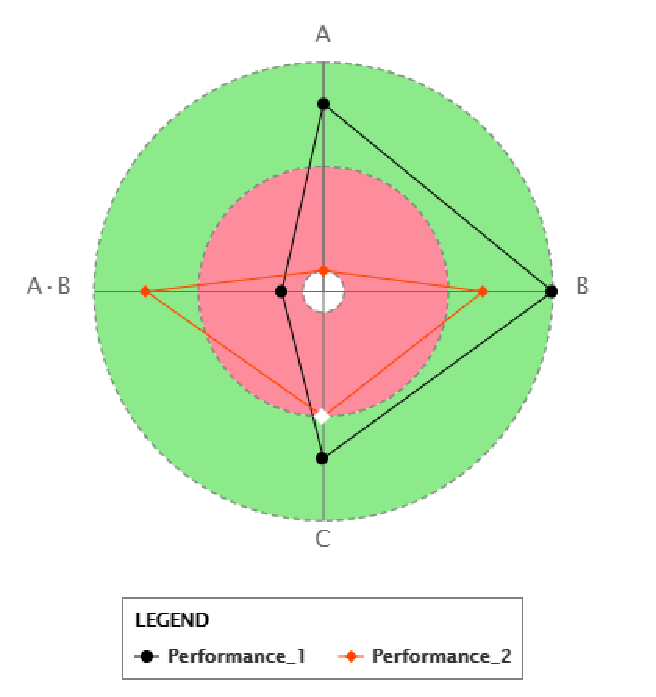
\includegraphics[width=10cm,height=10cm,keepaspectratio,]{pics/radar_plot.pdf}
\caption[The Radar Plot]{The radar Plot visualization for two performance-influence models, $\prod_1$ and $\prod_2$ with configuration options A, B, C and interaction A$\cdot$B.}
\end{figure}

The radar plot as shown in \hyperref[radaPlot]{Figure 2.1}, is one way of visually representing the performance-influence models. We use the normalized performance-influence models given in \hyperref[eq:2.3.5]{Equation 2.3.5} and \hyperref[eq:2.3.6]{Equation 2.3.6} for this example. The outer circle indicates +1, the most inner circle indicates -1, and the middle circle indicates 0, which corresponds to negative influence, positive influence and zero or no influence respectively. The underlying grey axis lines indicate configuration options A, B, C and the interaction A $\cdot$ B. The performance influence from each configuration option and interaction are plotted on corresponding axis lines for every performance-influence model.

For the sake of simplicity, for this visualization and all other visualizations that follow, we have used A as a short-hand form for c(A).  Similarly, for other configuration options and interactions.

If the performance contributed by a configuration option or interaction is 0, then it is indicated by an empty white marker symbol on the middle circle as seen by the configuration option C for the second performance-influence model.

In \hyperref[radaPlot]{Figure 2.1}, the first performance-influence model, $\prod_1$ is plotted in black and the second performance-influence model, $\prod_2$ in red. We can see from the visualization concerning first performance-influence model, that configuration options A, B and C are plotted in the green area, which means they increase the performance of the system. The interaction A$\cdot$B is marked in the red area of the visualization, which indicates that it decreases the performance of the system because, in real world systems, there are configuration options with a small but relevant influence on an NFPs.

Similarly, for the second performance-influence model, we can see that the configuration option A lies in the red area of the visualization indicating that it decreases the performance of the system. Whereas, the configuration options B and the interaction A$\cdot$B are plotted in the green area of the visualization, which indicates that they increase the performance of the system. Configuration option C has no influence on the performance of the system; hence it is marked with a different marker symbol that stands out from others. This is done to immediately recognize the configuration options that cause no influence on the performance of the system.

From \hyperref[radaPlot]{Figure 2.1}, we can infer that option B causes the highest influence on the performance for the first performance-influence model and for the second performance-influence model, configuration option A causes highest influence on the performance of the system, though they both lie in green and red area respectively. 

\subsection{The Text Plot}

\begin{figure}[ht]
\centering
\label{textPlot}
 %- \textbf{Your title}\par\medskip
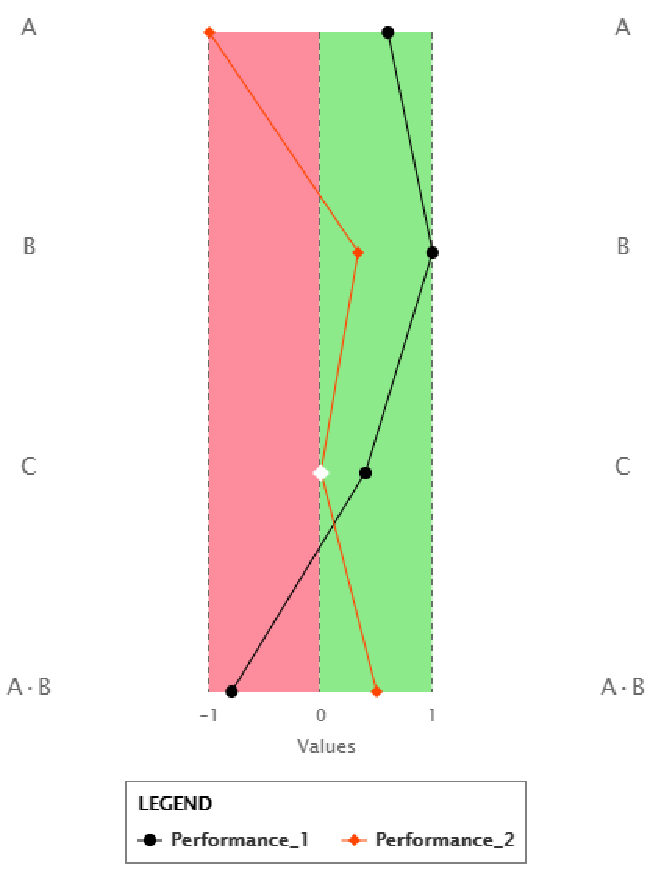
\includegraphics[width=12cm,height=13cm,keepaspectratio,]{pics/text_plot.pdf}
\caption[The Text Plot]{The text plot visualization for two performance-influence models, $\prod_1$ and $\prod_2$ with configuration options A, B, C and interaction A$\cdot$B.}
\end{figure}

The text plot as shown in \hyperref[textPlot]{Figure 2.2}, is the visual representation of the normalized performance-influence model in \hyperref[eq:2.3.5]{Equation 2.3.5} and \hyperref[eq:2.3.6]{Equation 2.3.6}. As shown in the \hyperref[textPlot]{Figure 2.2}, the left border line indicates -1, the middle line indicates 0 and the right line indicates +1, corresponding to positive, zero, and negative influence, respectively. 

This visualization technique and the color coding is perceived in a way similar to that of the radar plot. The black line indicates the first performance-influence model, $\prod_1$ and the red line indicates the second performance-influence model, $\prod_2$. 

From this visualization, we can easily infer that the configuration options plotted on the left and right lines are the ones that make highest influence on the system. For instance, for the first performance-influence model configuration option B makes highest influence on the performance of the system since it lies on the right line of the visualization. Similarly, for the second performance-influence model configuration option A makes the highest influence on the performance of the system, since it lies on the left line of the visualization.

The configuration option or interaction are marked on both the sides of the plot, hence this plot has the advantage of looking at the performance-influence models textually. This plot is easier for comparison of models, since the configuration options are vertically aligned than the radial form in the radar plot.

\subsection{The Ratio Plot}

\begin{figure}[ht]
    \centering
    \label{ratioPlot}
    %- \textbf{Your title}\par\medskip
   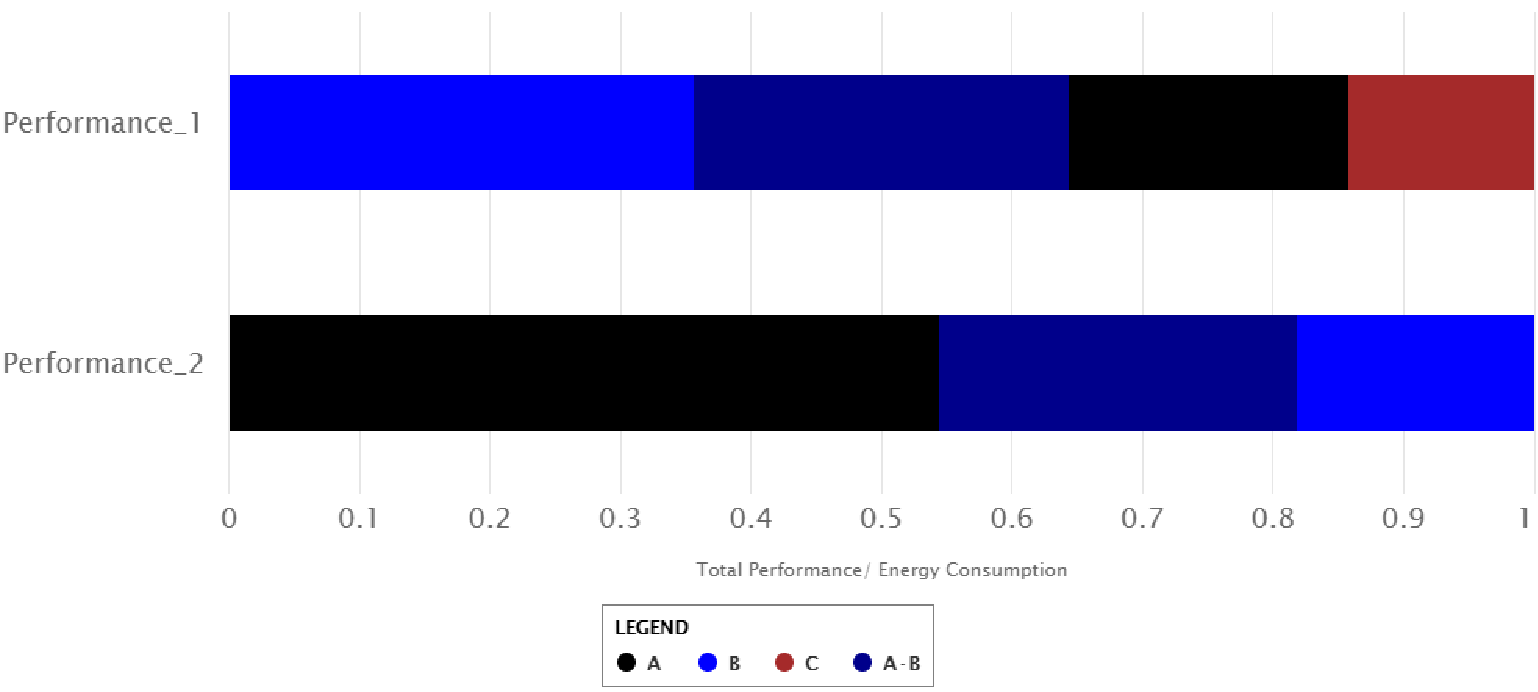
\includegraphics[width=15cm,height=15cm,keepaspectratio,]{pics/ratio_plot.pdf}
    \caption[The Ratio Plot]{The ratio plot visualization for two performance-influence models, $\prod_1$ and $\prod_2$ with configuration options A, B, C and interaction A$\cdot$B.}
\end{figure}


\begin{description}[leftmargin=0pt]
  \item[Normalization: ] For the ratio plot, we normalize the performance-influence models in a different way. We calculate the total performance of the system, it is the sum of all of the $\beta$ terms and is denoted mathematically as below:

\begin{equation*}
     \beta_{total} = \beta_{0} + \sum_{i \in \mathcal{O}}   {\beta_{\textit{i}}} + \sum_{i..j \in \mathcal{O}} {\beta_{\textit{i..j}}}
  \tag{2.3.7}\label{eq:2.3.7} 
\end{equation*}

After we obtain the $ \beta_{total}$, we normalize the performance-influence models, we divide the coefficient of every term per model with the $\beta_{total}$ of the corresponding model.

\begin{equation*}
  \prod {(c)} = \frac{\beta_{\mathrm{0}}}{\beta_{total}}  + \sum_{i \in \mathcal{O}} \frac{\beta_{\textit{i}}}{\beta_{total}} \cdot {c(i)} + 
 \sum_{i..j \in \mathcal{O}} 
 \frac{\beta_{\textit{i..j}}}{\beta_{total}} \cdot c(i)..c(j)
  \tag{2.3.8}\label{eq:2.3.8} 
\end{equation*}

I.e, we calculate the performance of individual configuration option or interaction with respect to the total performance to obtain the relative performance influence of the configuration options and interactions.

  
 For the performance-influence model in \hyperref[eq:2.3.1]{Equation 2.3.1}, we have the total performance i.e, $\beta_{total}$ = 14 units and we divide coefficient of every term by 14 to obtain the relative performance influence.

\begin{equation*}
  \prod_1{(c)} = 0.214 \cdot c(A) + 0.357  \cdot c(B) + 0.142 \cdot c(C) - 0.285 \cdot  c(A) \cdot c(B)
   \tag{2.3.9}\label{eq:2.3.9}
\end{equation*}

Similarly, for the performance-influence model in \hyperref[eq:2.3.2]{Equation 2.3.2}, we have the total performance influence i.e, $\beta_{total}$ = 11 units and the corresponding normalized performance-influence model is shown below:

\begin{equation*}
  \prod_2{(c)} = - 0.545 \cdot c(A) + 0.181 \cdot c(B) + 0.272 \cdot  c(A) \cdot c(B)
   \tag{2.3.10}\label{eq:2.3.10}
\end{equation*}

\item[Visualization: ] 
After obtaining the normalized performance-influence models, we sort the terms in descending order starting from the left side of the visualization regardless of the positive or the negative sign of the term. Hence the first bar represents the configuration option or interaction that makes the highest influence on the total performance of the system, the second bar makes the next highest influence on the total performance of the system and so on. As shown in the \hyperref[eq:2.3.10]{Equation 2.3.10}, the configuration option C for the second performance-influence model has no relevant performance influence, and therefore it does not appear in the ratio plot.

The Ratio plot as shown in \hyperref[ratioPlot]{Figure 2.3}, is the visual representation of the performance-influence models in \hyperref[eq:2.3.9]{Equation 2.3.9} and \hyperref[eq:2.3.10]{Equation 2.3.10}. The ratio plot represents the general influence that a configuration option or interaction has on the performance of the system, whereas the radar plot and the text plot show the positive and negative influence that a configuration option or interaction has on the performance of the entire system. 

We can see from the first performance-influence model, $\prod_1$ that configuration option B makes the highest influence and configuration option C makes the lowest influence on performance, regardless of it being positive or negative 

Similarly, for the second performance-influence model, $\prod_2$ we can see that the configuration option A makes the highest influence on the performance of the system, regardless of it being positive or negative. Configuration option B makes the least influence on the performance of the system and configuration option C makes no influence on the performance of the system. Hence, it does not appear in the visualization.

An advantage of this plot would be to check the overall influence a configuration option or interaction has on the performance of the system, irrespective of it being a positive or negative influence.

\end{description}